
\documentclass[a4paper]{article}
 \usepackage{indentfirst}
\usepackage[margin=1.9cm, top= 10mm]{geometry}
\usepackage{graphicx}

\begin{document}
\title{Assignment 1.1: Web Service (WDSL/SOAP)}
\author{
  \textbf{Bernardo Rui Andrade}\\
  12531650 \\
  \texttt{bernardo.andrade@tecnico.ulisboa.pt} \\
  \and
  \textbf{João Almeida}\\
 12531693\\
  \texttt{joao.santos.almeida@tecnico.ulisboa.pt} \\
}
\maketitle
\section*{Design and implementation description of the Calculator service}
The architecture of our Web Service is based on a Client-Server model. In this case, the service is stateless meaning that the client will only be allowed to make independent requests to the server. There is no Service Registry/Discovery component so the Client will be able to reach the Server in a hardcoded manner. The service interface is exposed by the Server through a contract such that the Client knows what type of requests the server accepts.\par
Our WSDL/SOAP Web Service was implemented using JAX-WS, Maven and Glassfish and following a Bottom-Up approach. First we designed and implemented our API (addition, substraction, multiplication and division). To generate the WSDL it was necessary to put "@WebMethod" annotations above the API methods that we wanted to be exposed. Then Maven, through the command "mvn install", generates the WSDL and all the inherent classes and deploys the service in Glassfish server.\par
The implementation of the Client passes through the generation of the service classes through the WSDL (obtained from an hardcoded endpoint) and the implementation of the request methods. 
\section*{Solution for making the Calculator service stateful}
A simple solution to maintain state (assuming multiple users) is adding an unique Client token/identifier to each request (e.g. with a SOAP handler we can attach it to the SOAP header/body of the message) sent to the service and then the server keeps the result of the operations/state in a key-value data store ($<$k,v$>$ = $<$Client UID, state$>$).  The client in his future requests has to decide between methods that will use the previous result/state or methods that don't require the previous result (like the stateless methods already defined in the previous service implementation).
\begin{figure}[h]
    \centering
    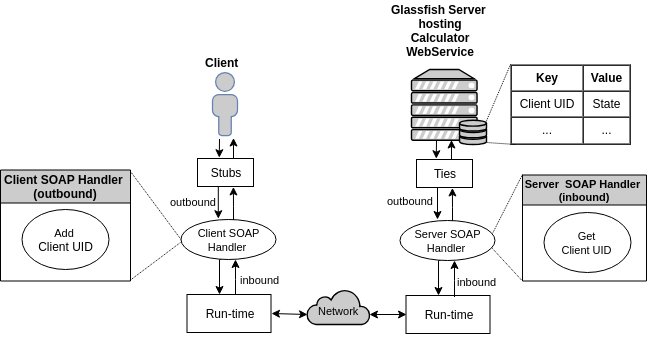
\includegraphics[scale=0.75]{assignment1-1}
    \caption{Stateful webservice solution siagram}
\end{figure}
\end{document}